\section{Experimental Setup}\label{sec:setup}

The results reported below retain the historical evaluator and caches. The corrected study is stored separately and applies a common external evaluator to every method, with both multiplication weights. Its equal-evaluation arm includes term-count and representation-node ablations. Historical energy measurements are kept separate from these newly selected models.

\subsection{Examples}
The study uses the regression examples distributed with the \texttt{mggp} package~\cite{mggpy}
(Table~\ref{tab:setup}, Fig.~\ref{fig:data}); the classification mode of the package returns a single objective and is
not considered. Example E1 is the tutorial system
\begin{equation}
y(k)=0.65\,y(k-1)+0.35\,u(k)+0.10\,u(k)\,y(k-1),
\label{eq:tutorial}
\end{equation}
excited by $u=\sin t+0.25\sin 3t$ over $300$ samples, of which the first $70\%$ are used for identification and the
remainder for validation. Example E2 adds white Gaussian measurement noise with standard deviation $0.02$ to the
output of E1. Example E3 uses the package simulator of the Bouc--Wen hysteresis model~\cite{IR2007}, $y=d_p u-h$ with
$\dot h=A\dot u-\beta|\dot u|h-\gamma\dot u|h|$, $A=0.9$, $\beta=\gamma=0.008$ and $d_p=1.6$, integrated by fourth-order
Runge--Kutta with a step of $1$~ms. Identification uses a $1$~Hz sinusoid whose amplitude grows linearly from $20$ to $50$
over $6$~s, and validation a $0.8$~Hz sinusoid of amplitude $45$ over $4$~s; both are decimated by $20$.

\begin{table}[!htbp]
\centering
\caption{Examples and search settings; $C_\mathrm{ref}$ for $\rho=1$ (common: population 100, 50 generations, crossover 0.9, initial mutation 0.2; baseline elite retention 10\%, multiple-shooting horizon $K=20$, primitives \texttt{mul} and $q^{-j}$).}
\label{tab:setup}
\setlength{\tabcolsep}{4pt}
\begin{tabular}{lcccccc}
\toprule
Example & $N_\mathrm{id}$ & $N_\mathrm{val}$ & genes & height & $j_{\max}$ & $C_\mathrm{ref}$ \\
\midrule
E1 Tutorial (noise-free) & 210 & 90 & 5 & 2 & 2 & 25 \\
E2 Tutorial (noisy) & 210 & 90 & 5 & 2 & 2 & 25 \\
E3 Bouc--Wen hysteresis & 300 & 200 & 8 & 3 & 3 & 72 \\
\bottomrule
\end{tabular}
\end{table}


\begin{figure*}[t]
\centering
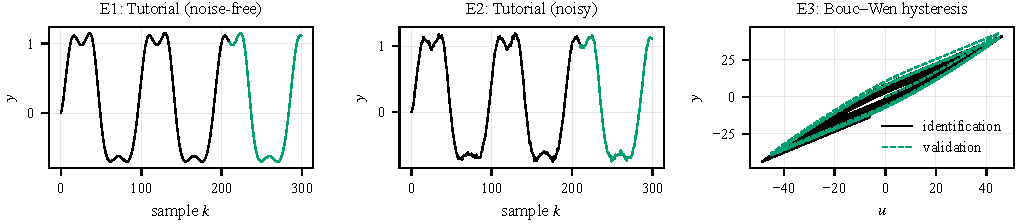
\includegraphics[width=\textwidth]{figures/fig_data.pdf}
\caption{Identification and validation data of the three examples. E3 is shown in the input--output plane, where the
loops reveal the hysteresis.}
\label{fig:data}
\end{figure*}

\subsection{Compared methods and protocol}
Three configurations share the representation, operators, initial rates and population/generation settings of Table~\ref{tab:setup}:
SO, the single-objective package minimising $J_E$, which returns its best model;
MO-lex, the bi-objective package mode with $C_\rho$ in \eqref{eq:cost} as the second objective;
and the proposed Green MGGP. Each configuration is run with \nSeeds{} seeds per example under two multiplication
weights: the unit weight $\rho=1$, which is the primary operation-count setting, supported in scale by the historical execution times (Section~\ref{sec:energy}), and the bit-level Green-Box weight
$\rho_K=\rhoK$. SO does not use the cost during the search, so its runs are common to both settings. Unless stated
otherwise, the results refer to $\rho=1$. The returned set of each run
(one model for SO) is reduced to distinct structures, and each model is refitted on the identification data and
simulated in free run on the validation data, initialised with the first $n$ measured outputs.

The 50 recorded generations comprise the initial population and 49 evolutionary steps. With 10\% elite retention, SO and MO-lex generate 90 offspring per step, whereas Green generates 100 before union-based survival. Thus equal generation counts do not imply equal numbers of fitness evaluations; the actual number also depends on reuse of valid fitness values. The mutation probability starts at 0.2 and follows the package's adaptive schedule, increasing by 0.1, up to 0.9, at nine-generation checkpoints when improvement is below 5\%. Elite retention of 10\% applies to the baselines; Green uses elitist union-based survival.

Each returned set is assessed by its hypervolume~\cite{ZT1999} in the normalised plane whose axes are $C/C_\mathrm{ref}$ and NRMSE,
with reference point $(1,1)$, where $C_\mathrm{ref}$ is the cost of $G$ genes of the maximum degree $2^{h_{\max}}$
(Table~\ref{tab:setup}). $\mathrm{HV}_\mathrm{id}$ uses $J_E$ and $\mathrm{HV}_\mathrm{val}$ the free-run validation
NRMSE of the same models; points beyond the reference contribute nothing. The model $\mathcal M_\tau$ in \eqref{eq:tau}
is characterised by its cost $C_\tau$ and validation NRMSE. For E1 and E2 we also record whether $\mathcal M_\tau$
contains the three regressors of \eqref{eq:tutorial}. Green MGGP is compared with each baseline by two-sided
Mann--Whitney tests~\cite{MW1947} with Holm correction~\cite{Hol1979} over all comparisons, and effect sizes are
reported by the Vargha--Delaney statistic $A_{12}$~\cite{VD2000}. All runs were executed in Python 3.13 on a single
CPU core.
